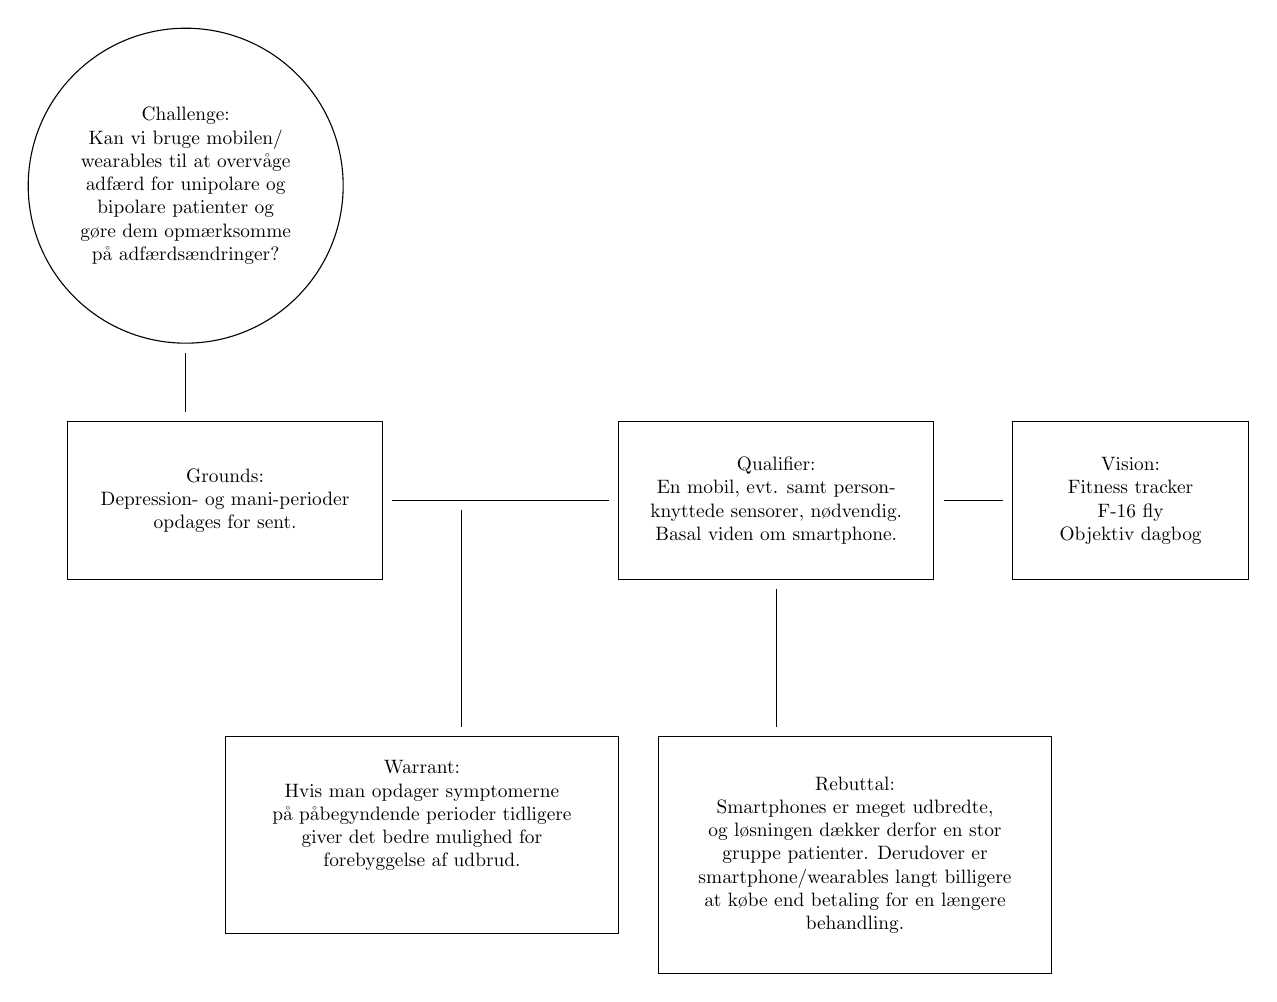
\begin{tikzpicture}

\draw  (-14,7) rectangle (-10,5);
\draw  (-12,3) rectangle (-7,0.5);
\draw  (-6.5,3) rectangle (-1.5,0);
\draw  (-7,7) rectangle (-3,5);
\draw  (-2,7) rectangle (1,5);

\node (v1) at (-10,6) {};

\node (v2) at (-7,6) {};
\draw  (v1) edge (v2);


\node (v3) at (-9,6) {};
\node (v4) at (-9,3) {};
\draw  (v3) edge (v4);
\node (v5) at (-5,3) {};
\node (v6) at (-5,5) {};
\draw  (v5) edge (v6);
\node (v7) at (-3,6) {};
\node (v8) at (-2,6) {};
\draw  (v7) edge (v8);



\draw  (-12.5,10) ellipse (2 and 2);
\node[align=center,scale=0.7] at (-12.5,10) {Challenge: \\Kan vi bruge mobilen/\\wearables  til at overvåge \\ adfærd for unipolare og \\ bipolare patienter og \\gøre dem opmærksomme\\ på adfærdsændringer?};

\node[align=center,scale=0.7] at (-12,6) {Grounds:\\Depression- og mani-perioder\\ opdages for sent.};
\node[align=center,scale=0.7] at (-9.5,2) {Warrant: \\Hvis man opdager symptomerne\\ på påbegyndende perioder tidligere\\ giver det bedre mulighed for\\ forebyggelse af udbrud.};

\node[align=center,scale=0.7] at (-5,6) {Qualifier:\\En mobil, evt. samt person-\\knyttede sensorer, nødvendig.\\ Basal viden om smartphone.};
\node[align=center,scale=0.7] at (-4,1.5) {Rebuttal:\\Smartphones er meget udbredte,\\ og løsningen dækker derfor en stor\\ gruppe patienter. Derudover er\\ smartphone/wearables langt billigere\\ at købe end betaling for en længere\\ behandling.};
\node[align=center,scale=0.7] at (-0.5,6) {Vision:\\Fitness tracker\\F-16 fly\\Objektiv dagbog};

\node (v10) at (-12.5,8) {};
\node (v9) at (-12.5,7) {};
\draw  (v9) edge (v10);
\end{tikzpicture}
    
    